\documentclass[tikz,border=4pt]{standalone}
\usepackage{amsmath}
\usetikzlibrary{arrows.meta}

\definecolor{signal}{RGB}{255,62,0}
\definecolor{meshfill}{RGB}{220,242,232}

\begin{document}
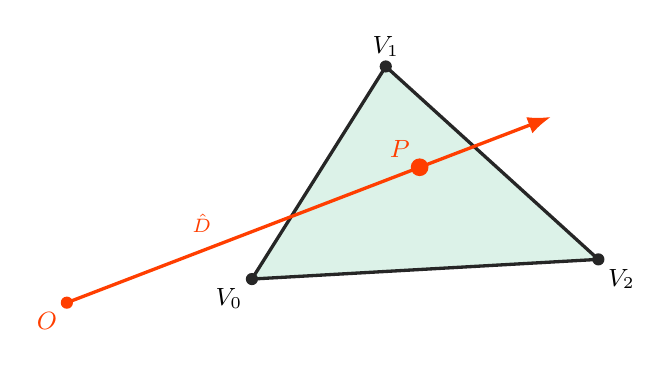
\begin{tikzpicture}[line cap=round,line join=round,>=Latex,font=\small]
  \coordinate (O) at (0,0);
  \coordinate (V0) at (2.35,0.30);
  \coordinate (V1) at (4.05,3.00);
  \coordinate (V2) at (6.75,0.55);
  \coordinate (P) at (4.48,1.72);

  \fill[meshfill] (V0) -- (V1) -- (V2) -- cycle;
  \draw[black!85,very thick] (V0) -- (V1) -- (V2) -- cycle;
  \draw[signal,very thick,->] (O) -- (6.15,2.36)
    node[pos=.32,above left,font=\scriptsize] {$\hat D$};

  \fill[signal] (O) circle (2.2pt);
  \fill[black!85] (V0) circle (2.2pt) (V1) circle (2.2pt) (V2) circle (2.2pt);
  \fill[signal] (P) circle (3.2pt);

  \node[below left,signal] at (O) {$O$};
  \node[above left,signal] at (P) {$P$};
  \node[below left] at (V0) {$V_0$};
  \node[above] at (V1) {$V_1$};
  \node[below right] at (V2) {$V_2$};
\end{tikzpicture}
\end{document}
